
\section{Linkstrecken}
\label{section:linkstrecken}
\begin{frame}%STARTCONTENT

\begin{columns}
    \begin{column}{0.48\textwidth}
    
\begin{figure}
    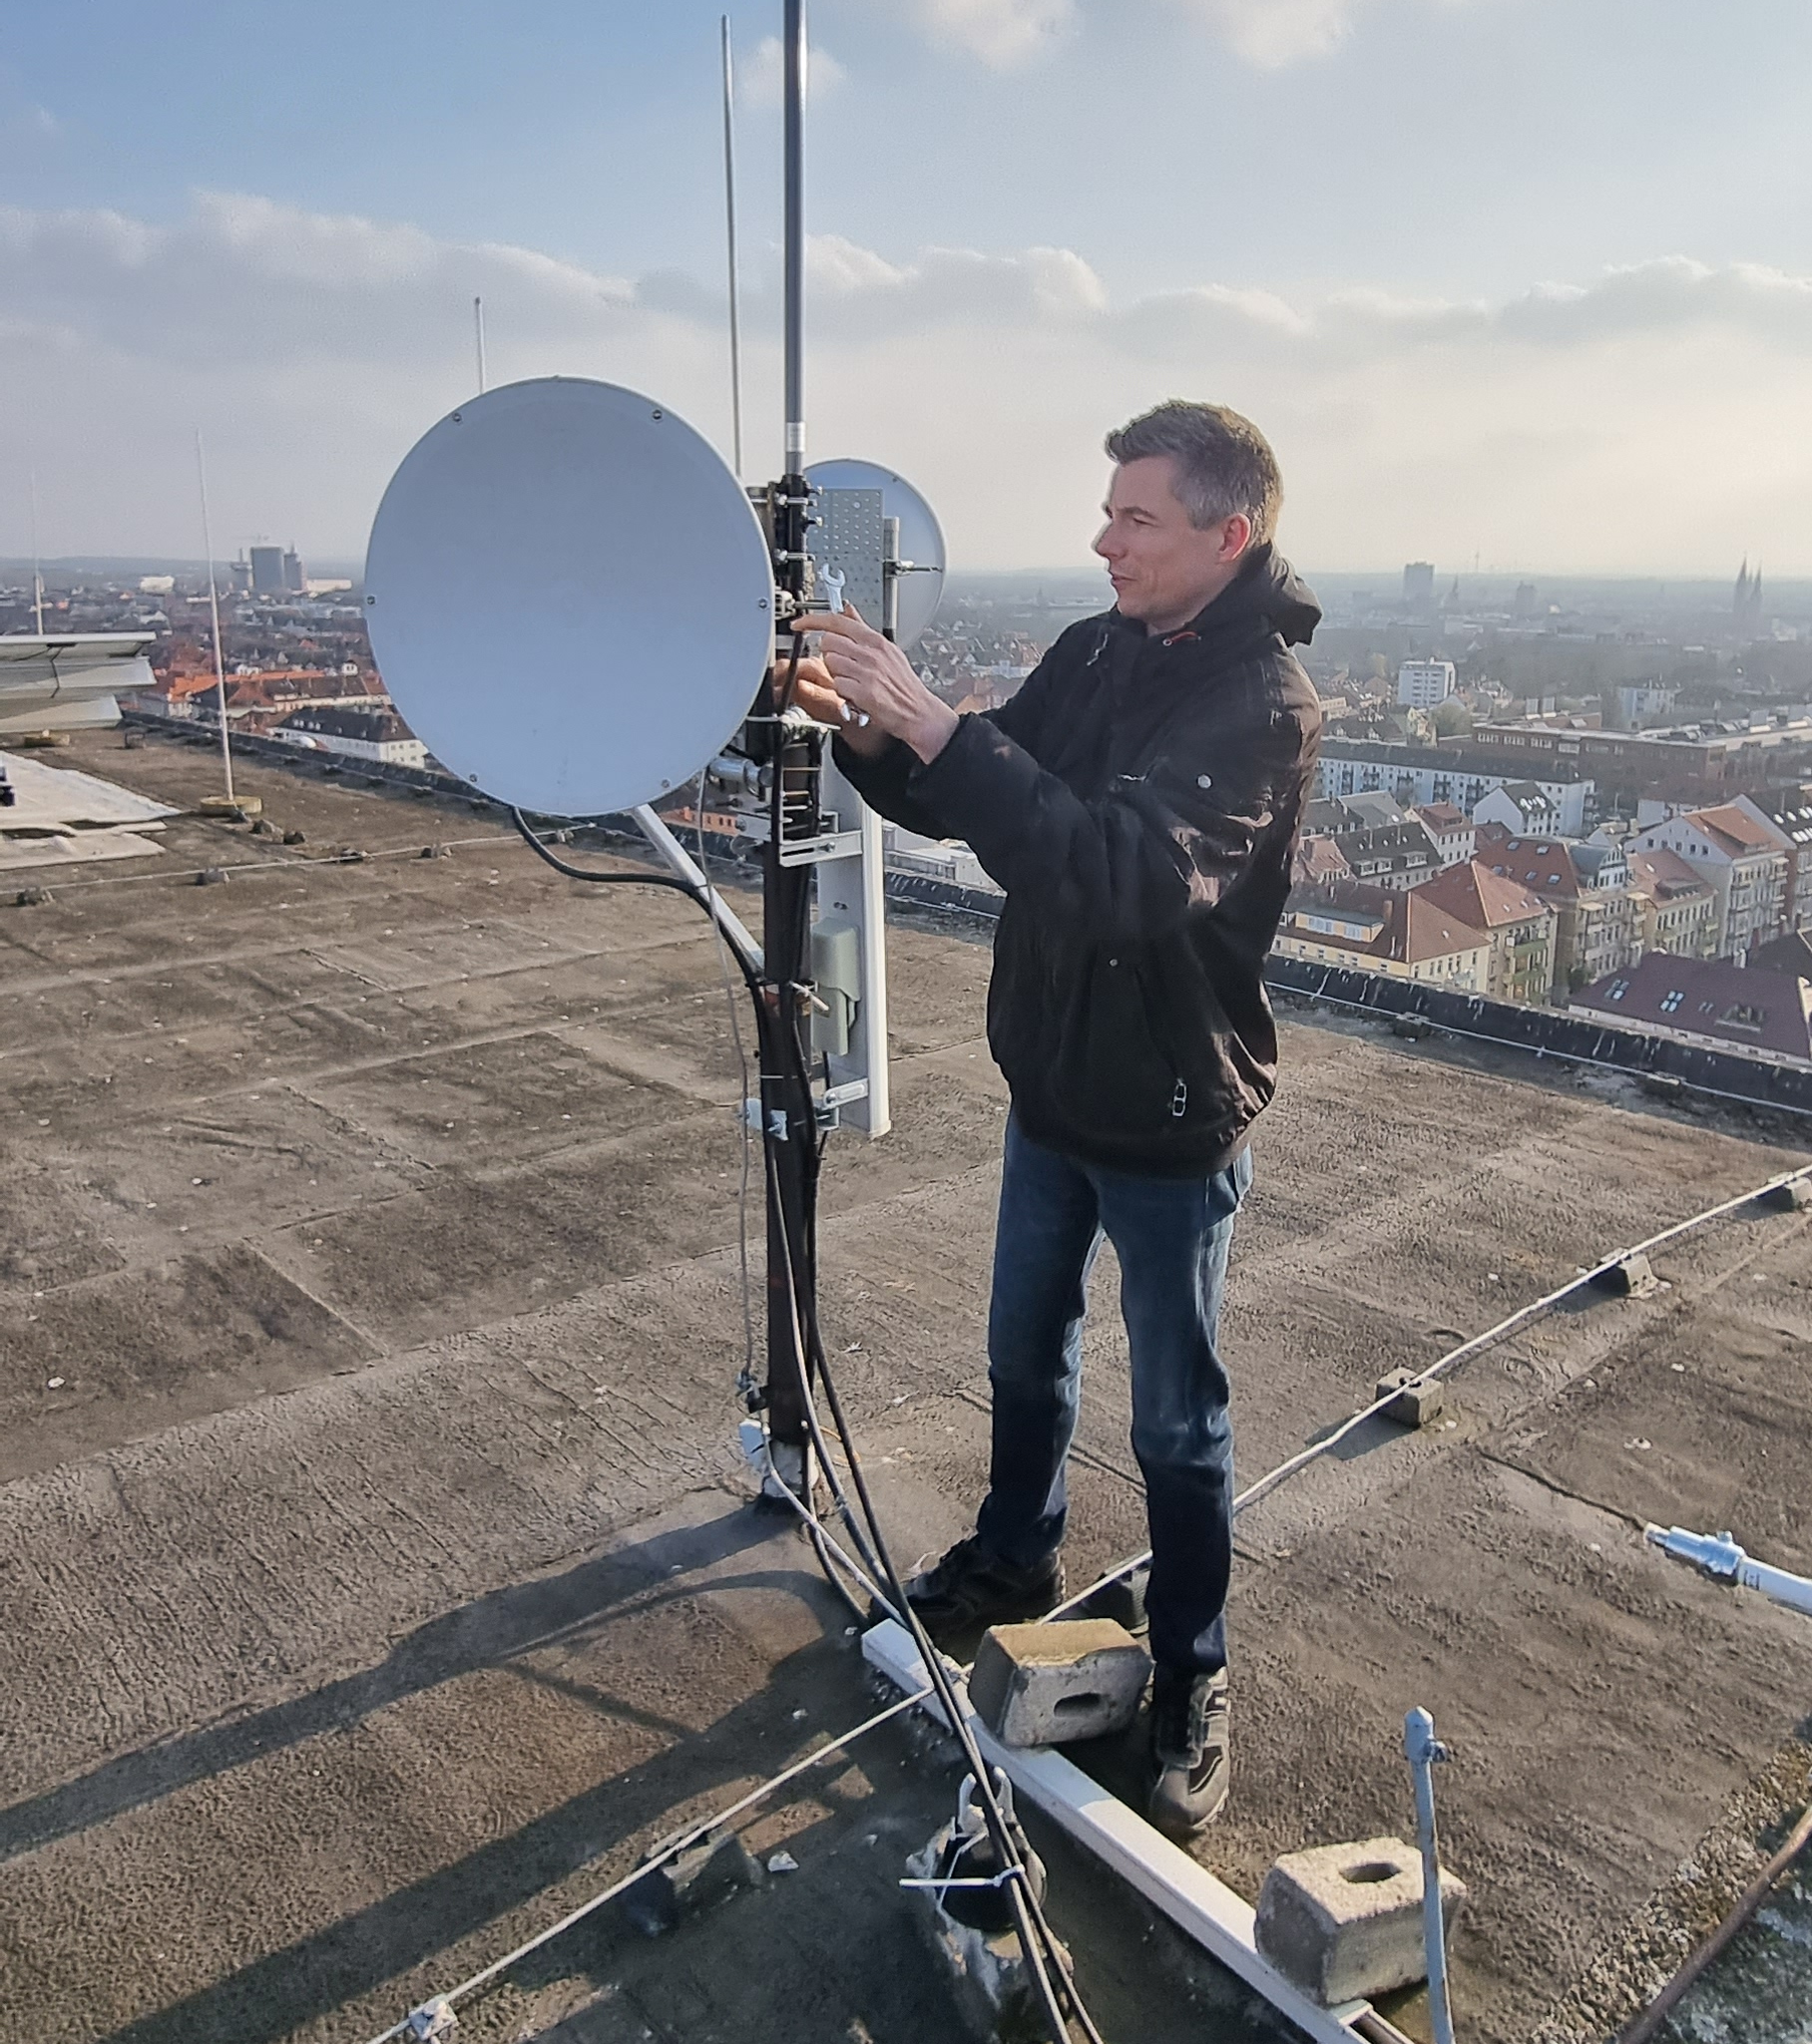
\includegraphics[width=0.85\textwidth]{foto/127}
    \caption{\scriptsize Wartungsarbeiten am HAMNET-Knoten DB0FC, im Vordergrund die Richtantenne für die Linkstrecke zu DB0BWL}
    \label{n_linkstrecken_db0fc}
\end{figure}

    \end{column}
   \begin{column}{0.48\textwidth}
       \begin{itemize}
  \item Fest eingerichtete Funkverbindung zwischen zwei Amateurfunkstellen
  \item Automatisch arbeitende Station
  \item Benötigt eigene Zulassung mit Rufzeichen durch BNetzA
  \end{itemize}

   \end{column}
\end{columns}

\end{frame}

\begin{frame}\begin{itemize}
  \item Überträgt in der Regel Daten
  \item Kann als analoge Brücke zwischen Relais dienen
  \item Arbeitet meistens im GHz-Bereich des Amateurfunk-Spektrums
  \item Bilden zusammen das HAMNET (Highspeed Amateurradio Multimedia NET-work)
  \end{itemize}

\end{frame}

\begin{frame}
\only<1>{
\begin{QQuestion}{NE405}{Was sind \glqq Linkstrecken\grqq{} und wozu dienen sie im Amateurfunk?}{Es sind Verbindungen zwischen unterschiedlichen Netzwerkprotokollen, z.~B. AX-25 und TCP/IP.}
{Es sind Einrichtungen, z.~B. bei Relaisfunkstellen oder Digipeatern, die eine Verbindungsherstellung über das Telefonnetz erlauben.}
{Es sind fest eingerichtete Funkverbindungen, z.~B. zur Vernetzung von Relaisfunkstellen oder mit einem HAMNET-Knoten.}
{Es ist eine Aufzählung von Links, z.~B. zu Amateurfunkseiten im HAMNET.}
\end{QQuestion}

}
\only<2>{
\begin{QQuestion}{NE405}{Was sind \glqq Linkstrecken\grqq{} und wozu dienen sie im Amateurfunk?}{Es sind Verbindungen zwischen unterschiedlichen Netzwerkprotokollen, z.~B. AX-25 und TCP/IP.}
{Es sind Einrichtungen, z.~B. bei Relaisfunkstellen oder Digipeatern, die eine Verbindungsherstellung über das Telefonnetz erlauben.}
{\textbf{\textcolor{DARCgreen}{Es sind fest eingerichtete Funkverbindungen, z.~B. zur Vernetzung von Relaisfunkstellen oder mit einem HAMNET-Knoten.}}}
{Es ist eine Aufzählung von Links, z.~B. zu Amateurfunkseiten im HAMNET.}
\end{QQuestion}

}
\end{frame}%ENDCONTENT
